\documentclass{article}

\usepackage[utf8]{inputenc}
\usepackage{graphicx}
\usepackage{listings}
\usepackage[a4paper, left=2cm, right=2cm, top=3cm, bottom=3cm]{geometry}
\usepackage{amsmath}
\title{Advaned Programming for HPC - Report 4}
\author{Dinh Anh Duc}

\begin{document}

\maketitle

\section*{Implementation}
\footnotesize\begin{lstlisting}

__global__ void grayscale2D(uchar3 *input, uchar3 *output, int width, int height) {
        int x = threadIdx.x + blockIdx.x + blockDim.x;
        int y = threadIdx.y + blockIdx.y + blockDim.y;
        if (x > width || y > height){
            printf("x, y are outside the width, height");
            return;
        }
        int tid = x + y * width; 
	    output[tid].x = (input[tid].x + input[tid].y + input[tid].z) / 3;
        output[tid].z = output[tid].y = output[tid].x;
}
void Labwork::labwork4_GPU() {
    // Calculate number of pixels
    int pixelCount = inputImage->width * inputImage->height;	
    //char *hostInput = inputImage->buffer; // Perfect version
    char *hostInput = (char*) malloc(inputImage->width * inputImage->height * 3); // Test version
    char *hostOutput = new char[inputImage->width * inputImage->height * 3]; // Test version
    outputImage = static_cast<char *>(malloc(pixelCount * 3));
    for (int j = 0; j < 100; j++) {     // let's do it 100 times, otherwise it$
        # pragma omp parallel for
        for (int i = 0; i < pixelCount; i++) {
            outputImage[i * 3] = (char) (((int) inputImage->buffer[i * 3] + 
            (int) inputImage->buffer[i * 3 + 1] + (int) inputImage->buffer[i * 3 + 2]) / 3);
            outputImage[i * 3 + 1] = outputImage[i * 3];
            outputImage[i * 3 + 2] = outputImage[i * 3];
        }
    }

    // Allocate CUDA memory    
    uchar3 *devInput;
    uchar3 *devOutput;
    //cudaMalloc(&devInput, pixelCount*3); // Perfect version
    cudaMalloc(&devInput, pixelCount * sizeof(uchar3)); // Test version
    //cudaMalloc(&devOutput, pixelCount*3); // Perfect version
    cudaMalloc(&devOutput, pixelCount * sizeof(float)); // Test version
    
    // Copy CUDA Memory from CPU to GPU
    //cudaMemcpy(devInput, hostInput, pixelCount*3, cudaMemcpyHostToDevice); // Perfect version
    cudaMemcpy(devInput, hostInput, pixelCount * sizeof(uchar3), cudaMemcpyHostToDevice); // Test version


    // Processing
    dim3 blockSize = dim3(32, 32);
    dim3 gridSize = ((int) ((inputImage->width + blockSize.x - 1)/blockSize.x), (int)((inputImage->height + blockSize.y - 1)/blockSize.y));
    grayscale2D<<<gridSize, blockSize>>>(devInput, devOutput, inputImage->width, inputImage->height);

    // Copy CUDA Memory from GPU to CPU
    //cudaMemcpy(outputImage, devOutput, pixelCount*3, cudaMemcpyDeviceToHost); // Perfect version 
    cudaMemcpy(hostOutput, devOutput, pixelCount*sizeof(float), cudaMemcpyDeviceToHost); // Test version

    // Cleaning
    //free(hostInput);
    cudaFree(devInput);
    cudaFree(devOutput);
}

\end{lstlisting}
\section*{Result}
\begin{figure}[h]
\center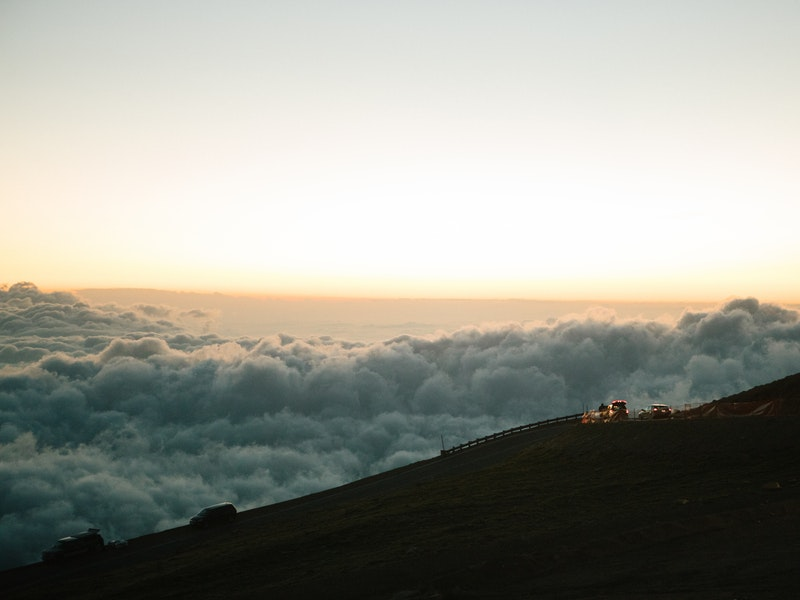
\includegraphics[scale=0.3]{./labwork/data/cloud.jpeg}
\caption{Original input image}
\end{figure}
\begin{figure}[h]
\center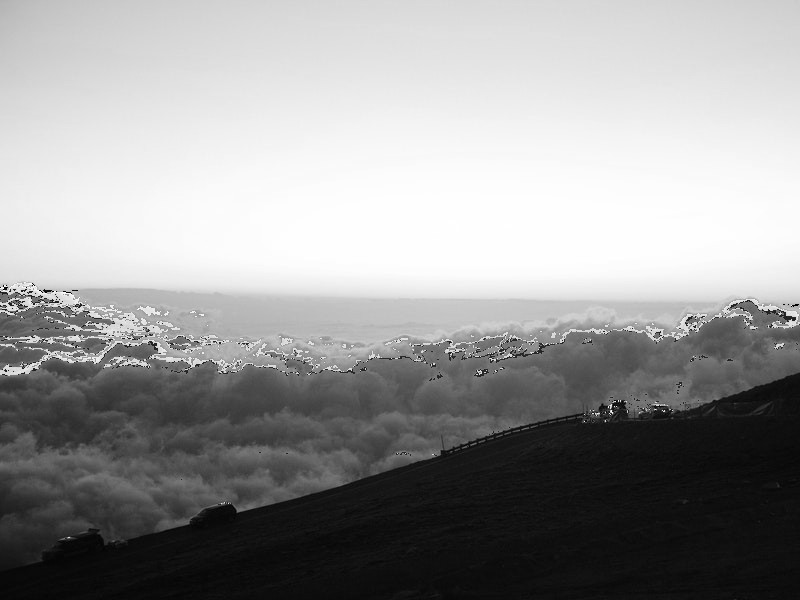
\includegraphics[scale=0.3]{./labwork/build/labwork4-gpu-out.jpg}
\caption{Output image}
\end{figure}
\newpage
\section*{Exercise}
\\
\textbf{Exercise 1:}
\\
Consider a GPU having the following specs (maximum numbers):
\\
\begin{itemize}
\item 512 threads/block
\item 1024 threads/SM
\item 8 blocks/SM
\item 32 threads/warp
\end{itemize}
\\
What is the best configuration for thread blocks to implement
grayscaling?
\\
\begin{itemize}
\item 8 x 8 
\item 16 x 16 
\item 32 x 32 
\end{itemize}
\\
\textbf{With 32 x 32 option:}
\begin{itemize}
\item 32 x 32 = 1024 \textgreater 512 threads/block (Out of limitation)
\item 1024 x 8 blocks/SM = 8192 \textgreater 1024 threads/SM (Out of limitation)
\end{itemize}
32 x 32 is not a good option
\\
\textbf{With 16 x 16 option:}
\begin{itemize}
\item 16 x 16 = 256 \textless 512 threads/block (Seem to be oke)
\item 256 x 8 blocks/SM = 2048 \textgreater 1024 threads/SM (Out of limitation)
\end{itemize}
\\
16 x 16 is not a good option
\\
\textbf{With 8 x 8 option:}
\begin{itemize}
\item 8 x 8 = 64 \textless 512 threads/block (Seem to be oke)
\item 64 x 8 blocks/SM = 512 \textless 1024 threads/SM (Seem to be oke)
\end{itemize}
\\
8 x 8 is not bad
\\
\textbf{Exercise 2:}
\\
Consider a device SM that can take max
\\
\begin{itemize}
\item 1536 threads
\item 4 blocks
\end{itemize}
\\
Which of the following block configs would result in the most
number of threads in the SM?
\\
\begin{itemize}
\item 128 threads/blk
\item 256 threads/blk
\item 512 threads/blk
\item 1024 threads/blk
\end{itemize}
\\
\textbf{With 128 threads/blk choice: }
\begin{itemize}
\item 128 x 4 blocks = 512 threads in a SM (Not a bad option)
\end{itemize}
\\
\textbf{With 256 threads/blk choice: }
\begin{itemize}
\item 256 x 4 blocks = 1024 threads in a SM (The best option)
\end{itemize}
\\
\textbf{With 512 threads/blk choice: }
\begin{itemize}
\item 512 x 4 blocks = 2048 threads in a SM (Out of limitation)
\end{itemize}
\\
\textbf{With 1024 threads/blk choice: }
\begin{itemize}
\item 1024 x 4 blocks = 4096 threads in a SM (Out of limitation)
\end{itemize}
\\
\textbf{Exercise 3:}
\\
Consider a vector addition problem
\begin{itemize}
\item Vector length is 2000
\item Each thread produces one output
\item Block size 512 threads
\end{itemize}
\\
How many threads will be in the grid?
\\
We need 2000 threads to execute 2000 sum opeations but we have 
maximum 512 threads in one block therefore we can use 4 blocks in 
a SM devices to calculate 2000 sum operations that means we will have
2048 threads in grid.
\\
\textbf{512 * 4 blocks/SM = 2048 threads (Not a bad option)}
\end{document}

